\documentclass[conference,onecolumn]{IEEEtran}

% Language setting
\usepackage[english]{babel}

\usepackage{ragged2e}

\IEEEoverridecommandlockouts
% The preceding line is only needed to identify funding in the first footnote. If that is unneeded, please comment it out.
\usepackage{cite}
\usepackage{amsmath,amssymb,amsfonts}
\usepackage{algorithmic}
\usepackage{graphicx}
\usepackage{textcomp}
\usepackage{xcolor}
\usepackage{blindtext}
\usepackage{float}
\usepackage{tabularx}
\usepackage{titlesec}
\usepackage{needspace}

\setlength{\abovedisplayskip}{4pt}
\setlength{\belowdisplayskip}{4pt}

\def\BibTeX{{\rm B\kern-.05em{\sc i\kern-.025em b}\kern-.08em
    T\kern-.1667em\lower.7ex\hbox{E}\kern-.125emX}}
\begin{document}

\title{Implementation of a Low-Level Digital Controller for DC Motors\\
{\footnotesize Laboratory 1}}

\author{\IEEEauthorblockN{Leonardo Achá Boiano}
\IEEEauthorblockA{\textit{Mechatronics Engineering: IMT 342} \\
\textit{Universidad Católica Boliviana}\\
Santa Cruz de la Sierra, Bolivia \\
leonardo.acha@ucb.edu.bo}
}

\maketitle
\justifying 

\begin{abstract}
This report presents the implementation of a low-level digital controller for DC motors in the context of a mechatronics engineering laboratory. The work addresses from the measurement of the input signal to the implementation and evaluation of the digital controller. The process of measuring the input signal, monitoring pulse-width modulation (PWM), and implementing open-loop control of the DC motor is described. In the second part of the laboratory, an open-loop system for the plant is developed, a PID controller in parallel configuration is designed and tuned, and the parameters are transferred to the real plant. The experimental results show the performance of the closed-loop system against different types of inputs, such as sinusoidal signals and steps. This work provides a comprehensive overview of the implementation of digital controllers for DC motors in mechatronic applications.

\end{abstract}

\begin{IEEEkeywords}
Control, Motor, ESP32, PID, Matlab, Open Loop, Closed Loop, Encoder.
\end{IEEEkeywords}

\section{Introduction}
This report presents the implementation of a low-level digital controller for DC motors in the context of a mechatronics engineering laboratory. This work focused on understanding and applying key concepts of control, pulse-width modulation (PWM), and closed-loop systems to optimize the performance and accuracy of the DC motor. Throughout the report, the stages of the experimental process are described, from the measurement of the input signal to the implementation and evaluation of the digital controller, providing a detailed view of this important area of mechatronics engineering.

\section{Procedure}
The methodology used in the laboratory was developed as follows. First, the input signal was measured via the wifi connection implemented in the microcontroller, in this case, the STM32. The input signal was sinusoidal and came from a program simulating an analog signal generator, sending the digitized signal with a 16-bit resolution.

Subsequently, the correct operation of the pulse-width modulation (PWM) module was monitored using an oscilloscope to ensure that the PWM generated the signal correctly with varied frequencies.

Then, the pulse control of the DC motor was implemented, which involved calculating the PWM duty cycle based on the input signal as shown in Figure~\ref{fig:encoder_signal}. Additionally, the direction of motor rotation was determined in relation to the ADC range, and the sign of the signal was provided separately.

The next step involved controlling the speed and direction of the motor, which was achieved by adjusting the PWM duty cycle.

To obtain the open-loop system's Bode Plot of phase and amplitude, the system's response to a step input was recorded, from which the system parameters were extracted.

In the second part of the laboratory, focused on building the closed-loop system, a digital controller was synthesized and implemented on the platform using the model previously obtained in the open-loop system to tune the controller in simulation. This controller was designed to meet technical specifications, including an overshoot of less than 30\% and a system error of e = 2° for a signal at 0.05 Hz.

Finally, the quality of the closed-loop system was evaluated to ensure it met the established technical requirements.

\section{Results}

\subsection{Plant Development}

\begin{figure}[H]
    \centering
    \resizebox{0.6\textwidth}{!}{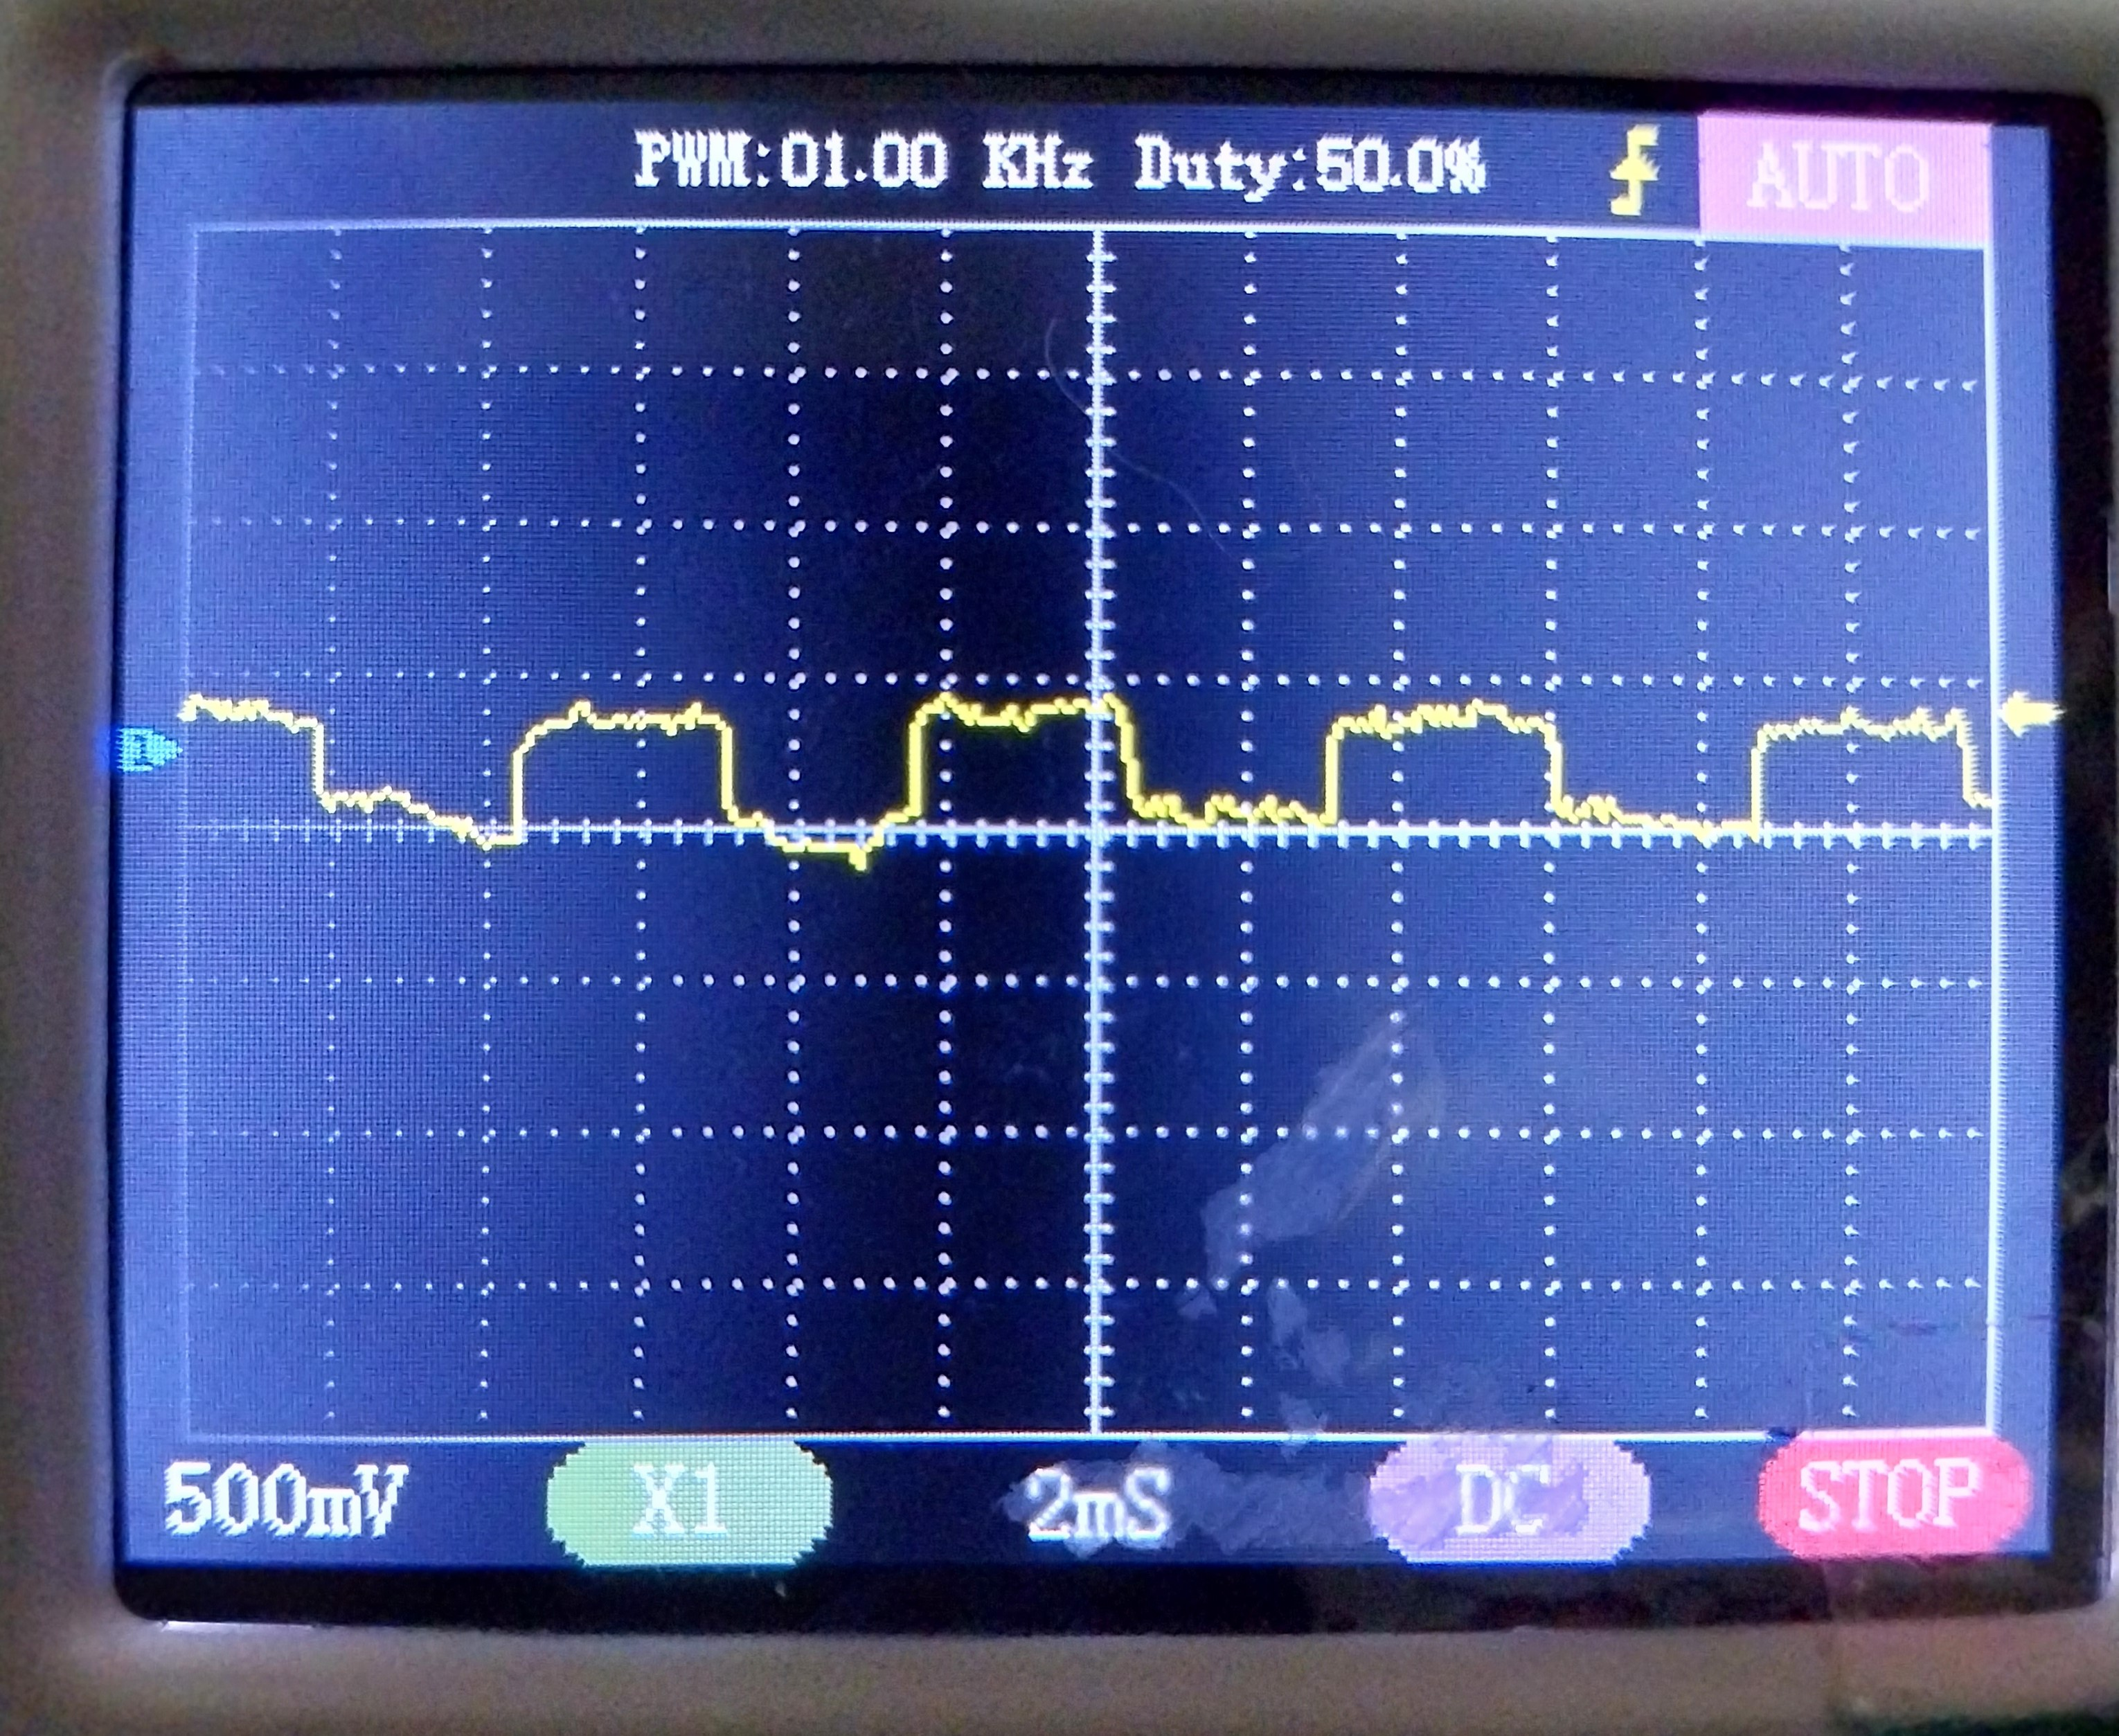
\includegraphics{images/Figure_1.jpg}}
    \caption{Encoder Signal of the Motor Visualized on the Oscilloscope}
    \label{fig:encoder_signal}
\end{figure}

Figure~\ref{fig:encoder_signal} shows the encoder signal of the DC motor, captured and visualized on an oscilloscope. This graphical representation is crucial for understanding how the motor's position is translated into an electrical signal. The waveform displayed on the oscilloscope provides information about the speed and direction of the motor, which is essential for the control and monitoring of the system. It was experimentally calculated that the encoder of the motor used generated an average of 480 pulses per revolution. This number was approximated to 512 to be a power of 2, as is often the case with binary encoders.

\begin{figure}[H]
    \centering
    \resizebox{0.6\textwidth}{!}{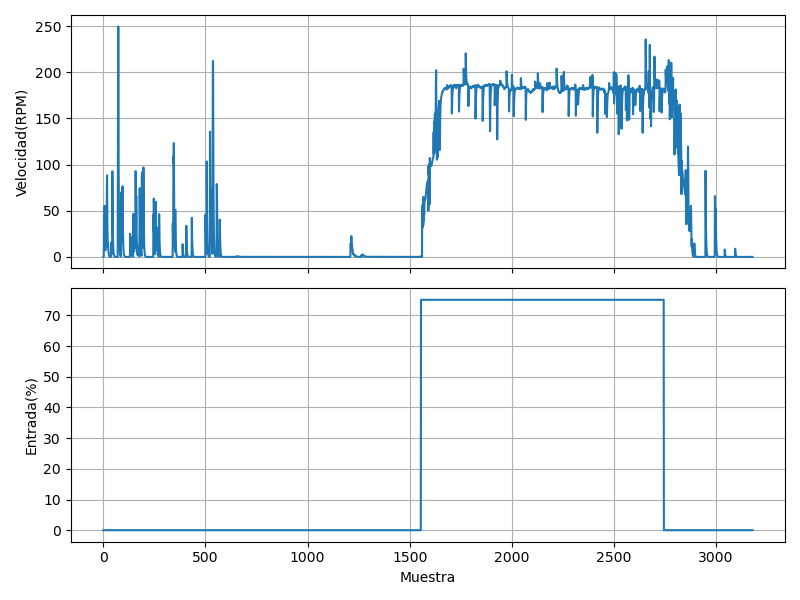
\includegraphics{images/Figure_2_ewma_filter_04.png}}
    \caption{Open-loop System Response to a Step Input}
    \label{fig:open_loop_response}
\end{figure}

Figure~\ref{fig:open_loop_response} shows the open-loop system's response to a step input. This graph is essential to understand the intrinsic behavior of the plant without any applied controller. It reveals aspects such as response time, overshoot, and the system's inherent stability. Note that the initially measured signal exhibited a significant amount of noise. To mitigate this noise, a digital weighted moving average filter was implemented.

\subsection{System Identification}

\begin{figure}[H]
    \centering
    \resizebox{0.6\textwidth}{!}{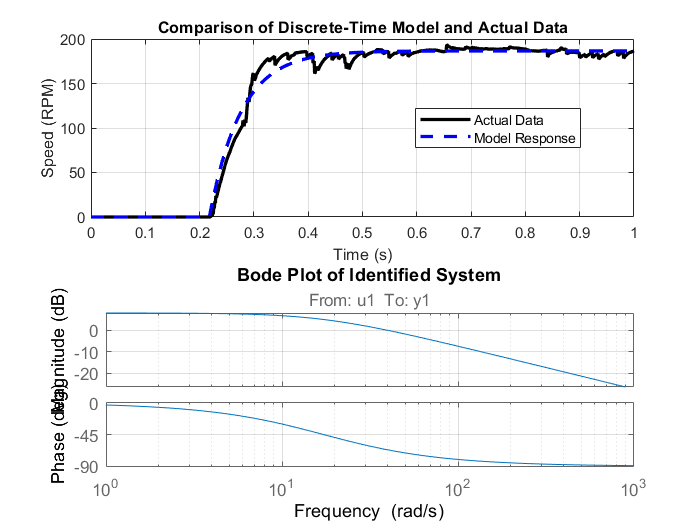
\includegraphics{images/Figure_3.png}}
    \caption{System Identification}
    \label{fig:sistem_identification}
\end{figure}

Figure~\ref{fig:sistem_identification} presents the system identification process. 
Using Matlab's system identification, the plant parameters were identified and the same was discretized using the zero-order hold method.
Through this procedure, the characteristic parameters of the plant are obtained, including its frequency response and dynamics.

\begin{equation}
\frac{0.04234 z^{-1}}{1 - 0.983 z^{-1}}
\end{equation}


\subsection{Controller Implementation}

Once the system was identified, we proceeded to select a controller. In this case, we opted for the PID controller in parallel configuration due to its ease of being tuned using practical methods without requiring complex calculations. As shown in the following equations, the Tustin approximation was used to discretize this controller. Then, the controller parameters were fine-tuned through simulation. Finally, the parameters were transferred to the plant, correcting the inherent discrepancies between the simulated model and the real plant to minimize errors.

\begin{align}
C(s) &= K_p + \frac{K_i}{s} + K_d s \label{eq:1} \\
s &= 2T_s \cdot \frac{z - 1}{z + 1} \label{eq:2} \\
C(s) &= \frac{U(s)}{E(s)} = K_p + \frac{K_i}{\frac{2}{T_s} \cdot \frac{z - 1}{z + 1} + K_d \cdot \frac{2}{T_s} \cdot \frac{z - 1}{z + 1}} \label{eq:3} \\
C(s) &= \frac{2(z - 1)(z + 1)K_pT_s + KiT_s^2(z + 1)^2 + 4Kd(z - 1)^2}{2(z - 1)(z + 1)T_s} \label{eq:4} \\
a &= 2K_pT_s \label{eq:5} \\
b &= KiT_s^2 \label{eq:6} \\
c &= 4K_d \label{eq:7} \\
d &= 2T_s \label{eq:8} \\
\frac{U(z)}{E(z)} &= \frac{2(z - 1)(z + 1)K_pT_s + KiT_s^2(z + 1)^2 + 4Kd(z - 1)^2}{2(z - 1)(z + 1)T_s} \label{eq:9} \\
\frac{U(z)}{E(z)} &= \frac{a(z - 1)(z + 1) + b(z + 1)^2 + c(z - 1)}{2d(z - 1)(z + 1)} \label{eq:10} \\
\frac{U(z)}{E(z)} &= \frac{az^2 - a + bz^2 + 2bz + b + cz^2 - 2cz + c}{d(z^2 - 1)} \label{eq:11} \\
\frac{U(z)}{E(z)} &= \frac{(a + b + c)z^2 + 2(b - c)z + (b + c - a)}{d(z^2 - 1)} \label{eq:12} \\
\frac{U(z)}{E(z)} &= \frac{(a + b + c) + 2(b - c)z^{-1} + (b + c - a)z^{-2}}{d(1 - z^{-2})} \label{eq:13} \\
u(k) &= \frac{(a + b + c)}{d}e(k) + \frac{2(b - c)}{d}e(k - 1) + \frac{(b + c - a)}{d}e(k - 2) + u(k - 2) \label{eq:14}
\end{align}


\begin{figure}[H]
    \centering
    \resizebox{0.6\textwidth}{!}{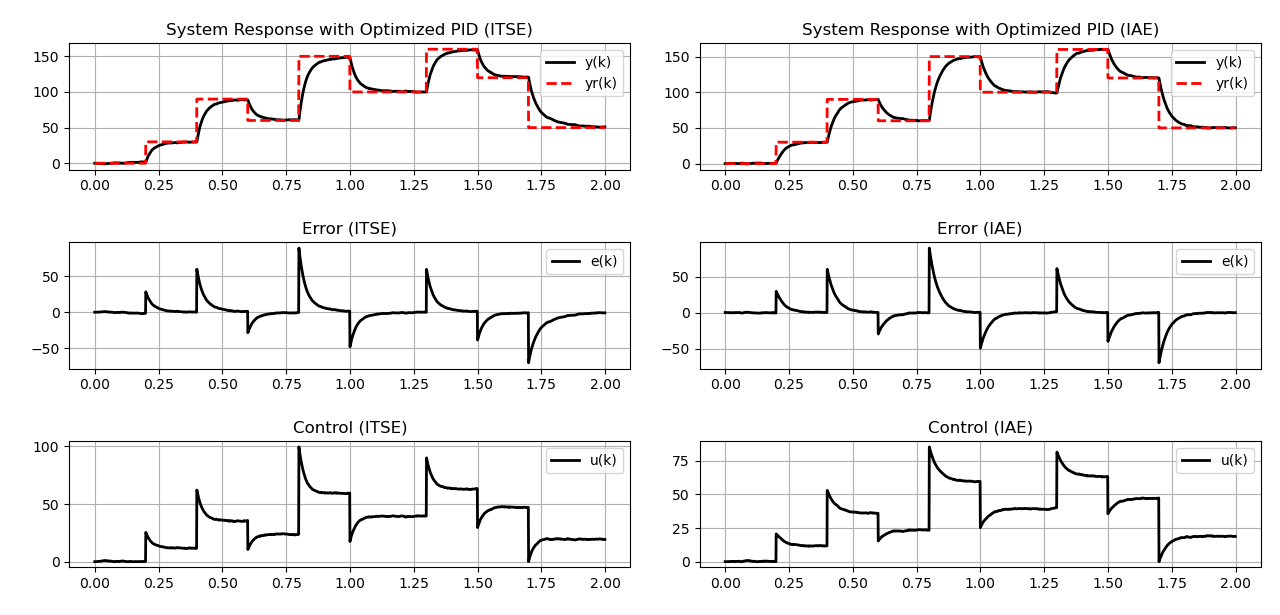
\includegraphics{images/Figure_4.png}}
    \caption{Closed-loop System Simulation to a Step Input}
    \label{fig:close_loop_response_simulation}
\end{figure}

Figure~\ref{fig:close_loop_response_simulation} illustrates the closed-loop system simulation in response to a step input. This simulation is crucial to evaluate and refine the behavior of the controlled system before implementing it on the physical plant. It provides an anticipated view of how the real system will respond under control.

\begin{figure}[H]
    \centering
    \resizebox{0.6\textwidth}{!}{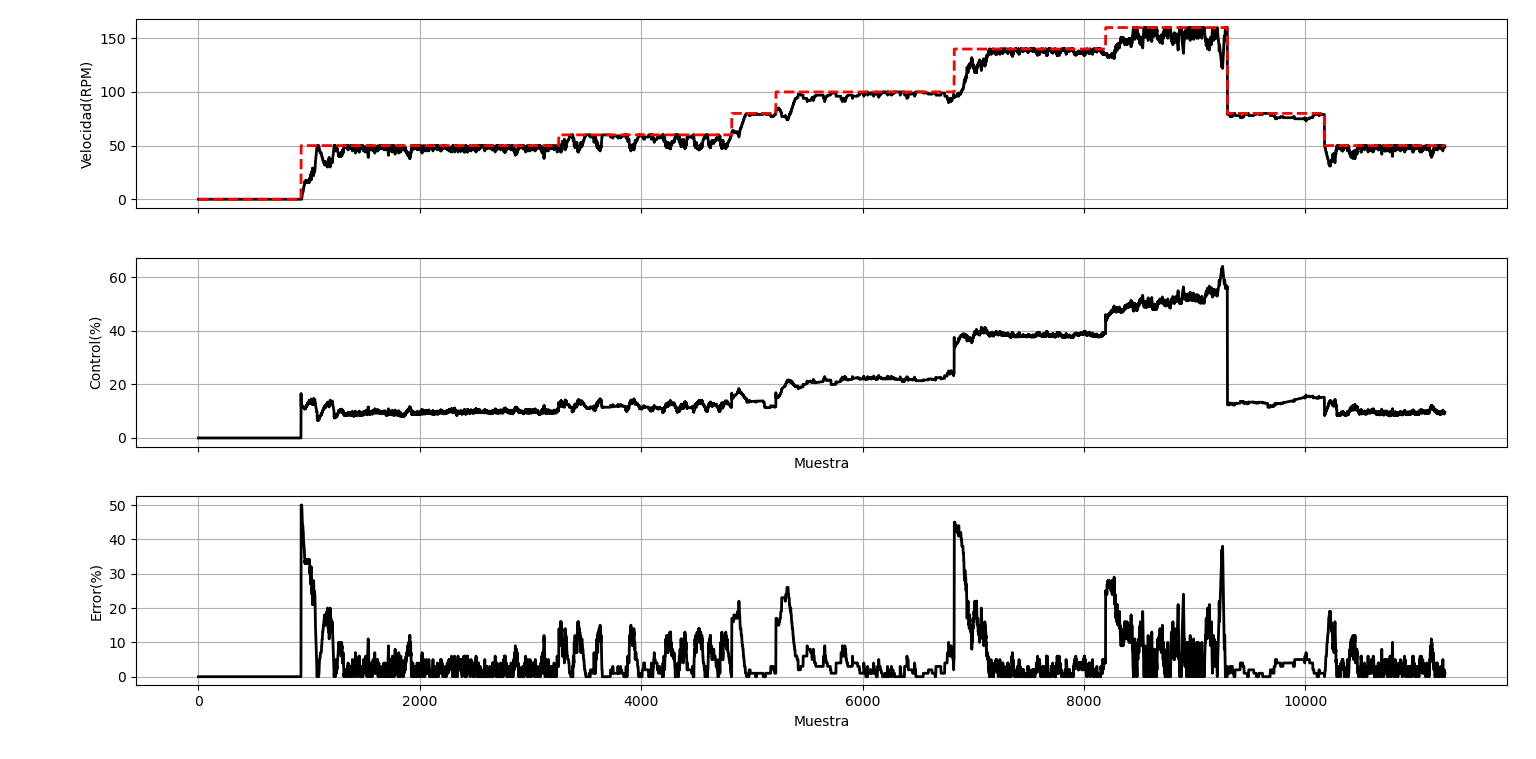
\includegraphics{images/Figure_5.png}}
    \caption{Controller Parameter Calibration with the Plant in Operation}
    \label{fig:close_loop_pid_calibration}
\end{figure}
Figure~\ref{fig:close_loop_pid_calibration} describes the process of calibrating the controller parameters while the plant is in operation. This critical step ensures that the controller is optimally adjusted to the specific characteristics and dynamics of the real plant.

\begin{figure}[H]
    \centering
    \resizebox{0.6\textwidth}{!}{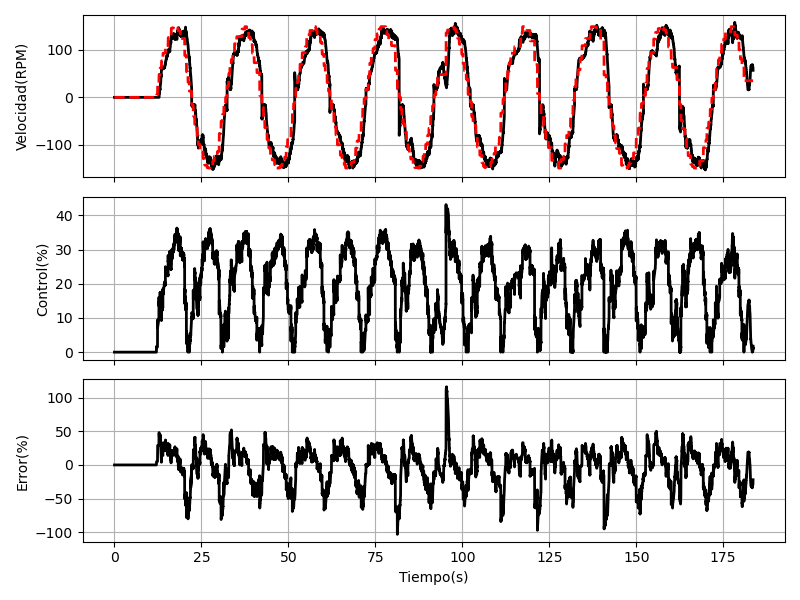
\includegraphics{images/Figure_6.png}}
    \caption{Closed-loop System Response to a Sinusoidal Input with a Frequency of 0.05 Hz}
    \label{fig:close_loop_sine_response}
\end{figure}

The analysis of the experimentally collected data shows that the phase lag of the developed system concerning a sinusoidal signal of 0.05 Hz is 1.24°, as observed in Figure~\ref{fig:close_loop_sine_response}.

\begin{figure}[H]
    \centering
    \resizebox{0.6\textwidth}{!}{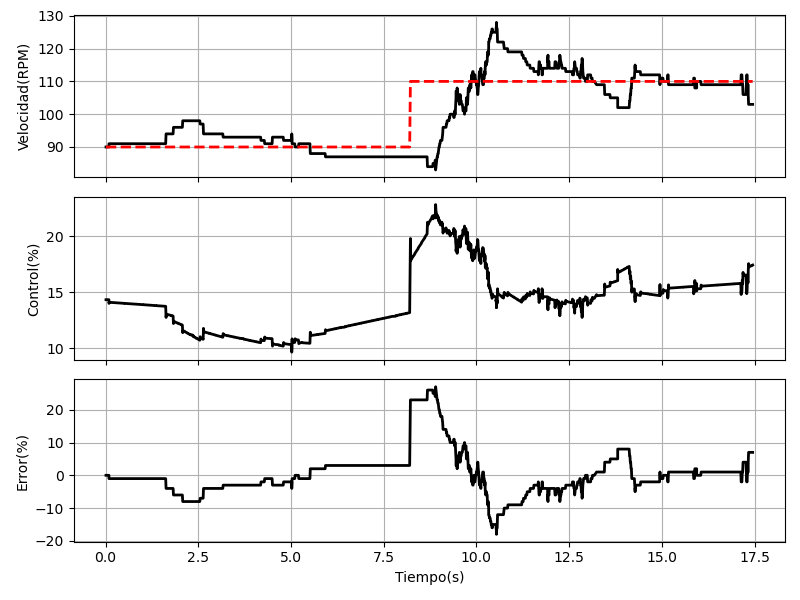
\includegraphics{images/Figure_7.png}}
    \caption{Closed-loop System Response to a Step Input}
    \label{fig:close_loop_step_response}
\end{figure}
Finally, the analysis of the step response for a change of 20 RPM shows an overshoot of 16.36\%, as seen in Figure~\ref{fig:close_loop_step_response}.

\section{Conclusion}
This report presented the implementation of a low-level digital controller for DC motors in the context of a mechatronics engineering laboratory. Several key stages have been addressed throughout the work, from the measurement of the input signal to the implementation and evaluation of the digital controller.

The experimental process began with the measurement of the input signal, which was a sinusoidal signal generated by an analog signal generator simulator program. Then, the pulse-width modulation (PWM) module's operation was monitored to ensure its correct functioning. Subsequently, the DC motor's pulse control was implemented, calculating the PWM duty cycle based on the input signal and the motor's rotation direction.

In the second part of the laboratory, an open-loop system for the plant was developed, obtaining its frequency response and dynamics. Then, a PID controller in parallel configuration was designed and tuned through simulation using the plant model. These parameters were transferred to the real plant after correcting the discrepancies between the model and the real plant.

The experimental results showed the closed-loop system's response to different types of inputs, such as sinusoidal signals and steps. A system phase lag of 1.24° and an overshoot of 16.36\% in the step response were observed, indicating that the digital controller achieves good performance in terms of reference tracking and stability.

In summary, this work provides a detailed view of the implementation of a low-level digital controller for DC motors in a mechatronics engineering laboratory environment. It has demonstrated the importance of system identification, controller tuning, and correcting discrepancies between the model and the real plant to achieve satisfactory control system performance.

\end{document}